\section{Data acquisition}

\subsection{Digitization}

Digitization differs from digitalisation. Digitization corresponds to the conversion from analogic to digital, while digitalisation corresponds to the development of electronics in society.

In order to digitize a signal, we have to operate an analog-to-digital conversion. A device used to perform this conversion is called an ADC. An ADC features two sub-operations:

\begin{itemize}
    \item Sampling (i.e. time discretization) : parameter = sampling frequency
    \item Quantization (i.e. amplitude discretization) $\rightarrow$ discrete steps : parameter = resolution
\end{itemize}

\subsubsection{Amplitude discretization (quantization)}



\begin{minipage}[c]{0.45 \linewidth}
\begin{figure}[H]
    \centering
    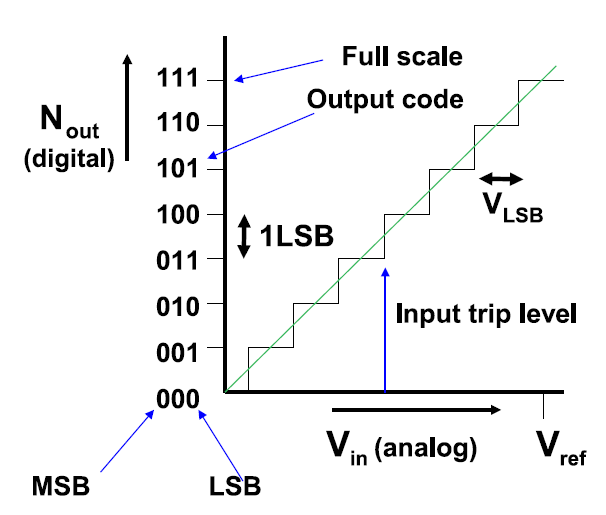
\includegraphics[width = 0.7 \textwidth]{L5/img/quantization2.PNG}
\end{figure}
\end{minipage}\hfill
\begin{minipage}[c]{0.45 \linewidth}
\begin{itemize}
    \item $2^N- 1$ decision levels
    \item Resolution: $LSB = \Delta = V_{FS}/2^N$
    \item Dynamic range: peak-to-peak signal $< 2^N \Delta $ 
    \item RMS quantization error = $V_{LSB}/\sqrt{12}$. Due to $e_{rms}^2 = \frac{1}{V_{LSB}}\int_{-V_{LSB}/2}^{V_{LSB}/2} v^2 \dif v = \frac{V_{LSB}^2}{12} $
\end{itemize}
\end{minipage}

\paragraph{Harmonic distortion}

Quantization is a distortion process. We see in the graph below that for small resolution (small $N$), the power of the high-order harmonics is still significant.
\begin{figure}[H]
    \centering
    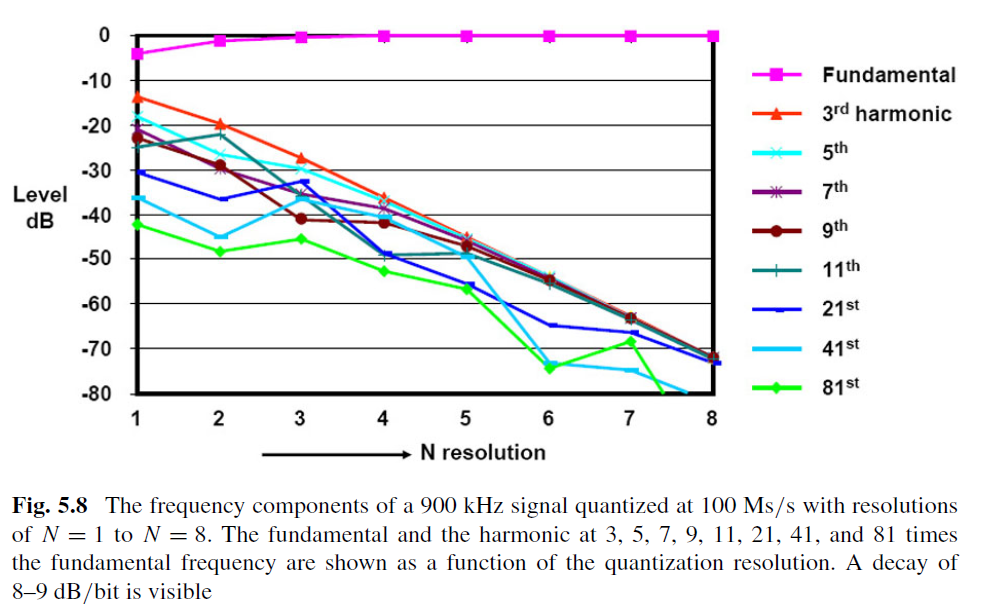
\includegraphics[width = 0.7 \textwidth]{L5/img/harmonic-distortion.PNG}
\end{figure}

\subsubsection{Time discretization (sampling)}

\begin{minipage}[c]{0.45 \linewidth}
\begin{figure}[H]
    \centering
    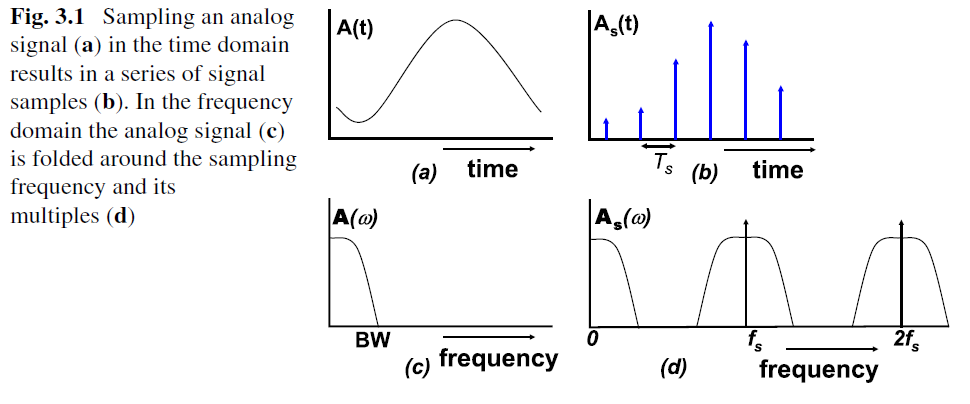
\includegraphics[width =  \textwidth]{L5/img/sampling.PNG}
\end{figure}
\end{minipage}\hfill
\begin{minipage}[c]{0.45 \linewidth}
Here, we see that sampling in the time domain leads to periodization in the frequency domain. The Nyquist criterion ($f_{S} > 2 f_{max,signal}$) needs to be respected in order to avoid aliasing (repli spectral).
Ideally, time and amplitude discretizations can
be interchanged.
\end{minipage}

\subsubsection{Quantization noise}

\begin{minipage}[l]{0.4 \linewidth}
\begin{figure}[H]
    \centering
    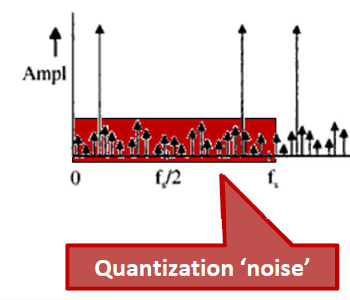
\includegraphics[width =  0.7\textwidth]{L5/img/quantization-noise.PNG}
\end{figure}
\end{minipage}\hfill
\begin{minipage}[c]{0.52 \linewidth}
Quantization noise is dependent from resolution. Increasing the resolution reduces the quantization noise.
Starting at 7-bit resolution, the thermal and quantization noises can be treated similarly, as white gaussian noise.
\end{minipage}

\subsubsection{Quantizer errors}

\paragraph{Offset and gain}
Offset and gain errors are typically
not critical in sensing
applications, they can be compensated
by calibration or digital post-processing.

\begin{minipage}[l]{0.45 \linewidth}
\begin{figure}[H]
    \centering
    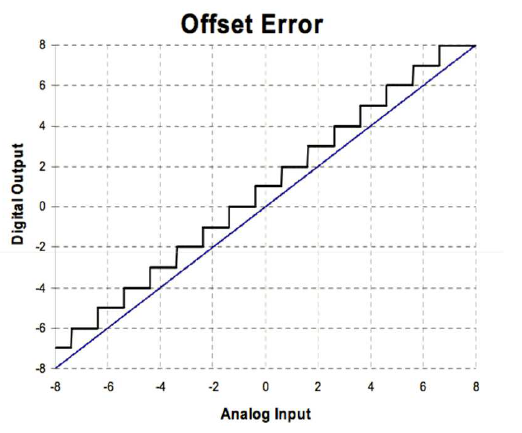
\includegraphics[width =  0.7\textwidth]{L5/img/offset.PNG}
\end{figure}
\end{minipage}\hfill
\begin{minipage}[c]{0.45 \linewidth}
\begin{figure}[H]
    \centering
    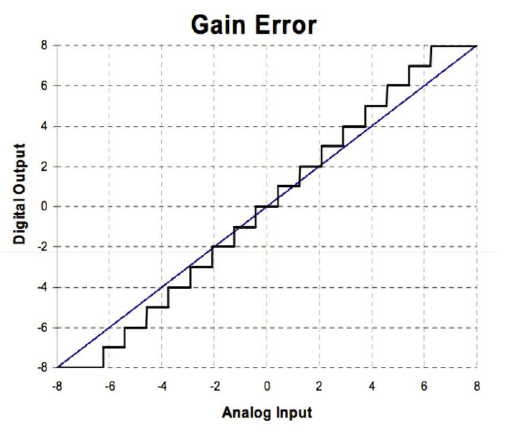
\includegraphics[width =  0.7\textwidth]{L5/img/gain.PNG}
\end{figure}
\end{minipage}

\paragraph{Non-monotonicity and DNL}

\begin{wrapfigure}[8]{r}{0.4\textwidth}
    \centering
    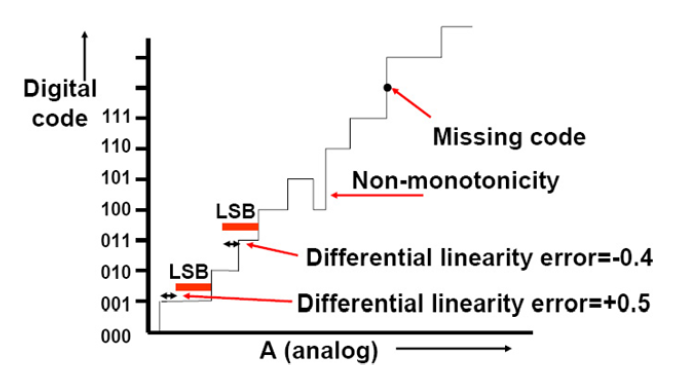
\includegraphics[width =  0.4\textwidth]{L5/img/DNL.PNG}
\end{wrapfigure}

A non-monotonicity appears when input increases (resp. decreases)
while the output code decreases (resp. increases). This is often problematic in control applications
(feedback gain changes sign).

A Differential Non Linearity (DNL) is the deviation of the actual step sizes from 1 LSB, defined as:
$$ DNL = \frac{V_{in}(Q_{m+1} - V_{in}(Q_m)}{V_{1LSB}} -1 $$

\paragraph{INL}
Integral Non Linearity (INL) is an accumulation of DNL errors. This translates into a deviation from the ideal curve in the analog domain expressed as \% of the full scale. We can reduce this effect with a linear calibration (better with polynomial calibration).

\begin{figure}[H]
    \centering
    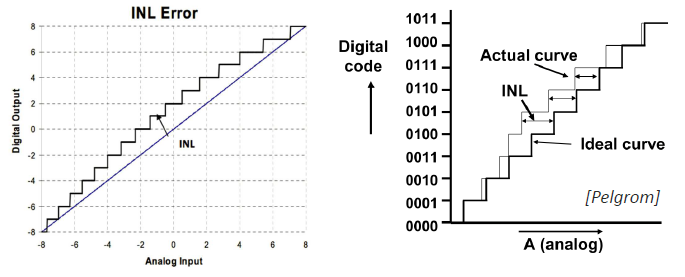
\includegraphics[width =  0.6\textwidth]{L5/img/INL.PNG}
\end{figure}


\subsection{ADC architectures}

\begin{figure}[H]
    \centering
    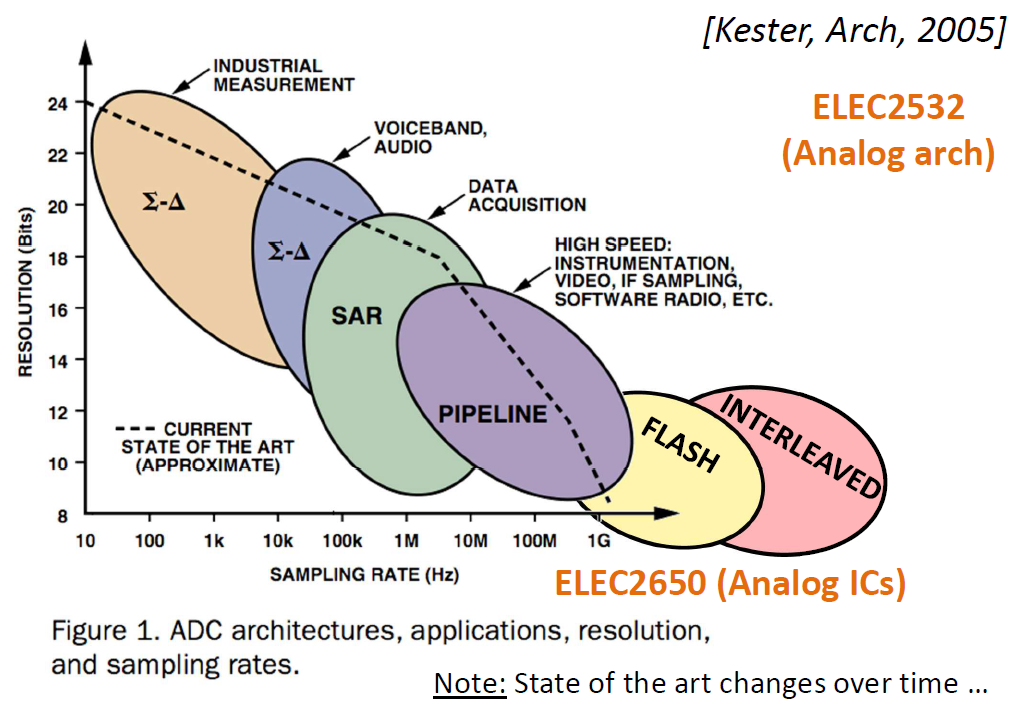
\includegraphics[width =  0.6\textwidth]{L5/img/architectures.PNG}
\end{figure}
\subsubsection{Flash ADC}

\begin{minipage}[c]{0.5\linewidth}
Flash converters are extremely fast compared to many other types of ADCs. A flash converter requires a huge number of comparators compared to other ADCs, especially as the precision increases. A flash converter requires $ 2^{N}-1$ comparators for an N-bit conversion. The size, power consumption and cost of all those comparators makes flash converters generally impractical for precisions much greater than 8 bits (255 comparators).

For 10 bits, we have 1023 decision levels, which is difficult to encode, slow, power consumer and very expensive. There is also a problem of resistance precision that leads to different decisions made from the comparators mainly because of the offset.
\end{minipage}\hfill
\begin{minipage}[c]{0.5 \linewidth}

\begin{figure}[H]
    \centering
    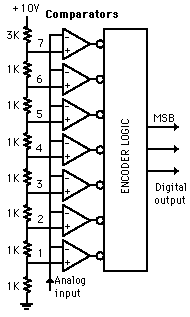
\includegraphics[width =  0.4\textwidth]{L5/img/flash-ADC.png}
\end{figure}

\end{minipage}

\subsubsection{Successive-AppRoximation (SAR) ADCs}

A SAR is a \textbf{high speed} (to
1 MHz throughput rates) and \textbf{high resolution} (16 bit and higher) ADC.
The conversion technique consists of comparing the unknown input $ V_{in}$ against
a precise voltage $V_a$ or current generated by a D/A converter. The conversion
technique is similar to a weighing process using a balance, with a set of N binary
weights (for instance, 1/2 kg, 1/4 kg, 1/8 kg, 1/16 kg, \dots up to total of 1 kg). Before
the conversion cycles, all the registers must be cleared and the comparator output
is high. The D/A converter has MSB (1/2 scale) at its inputs and generates an appropriate analog voltage $V_a$ equal to 1/2 of a full scale input signal. If the input is
still greater than the D/A voltage, the comparator remains high,
causing 1 at the register output. Then, the next bit (2/8 = 1/4 of FS) is tried.
If the second bit does not add enough weight to exceed the input, the comparator
remains high (1 at the output), and the third bit is tried. However, if the second
bit tips the scale too far, the comparator goes low resulting in 0 in the register,
and the third bit is tried. The process continues in order of descending bit weight
until the last bit has been tried. After the completion, the status line indicates the
end of conversion and data can be read from the register as a valid number
corresponding to the input signal. To sum up, this ADC acts as a \textit{floor} rounding, it returns the highest digital value that remains below the input signal.

\begin{minipage}[c]{0.45\linewidth}
\begin{figure}[H]
    \centering
    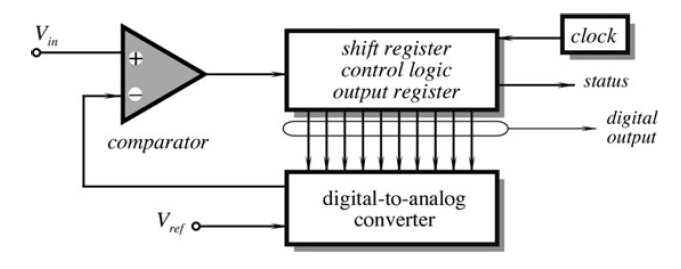
\includegraphics[width =  0.9\textwidth]{L5/img/SAR.PNG}
\end{figure}
\end{minipage}\hfill
\begin{minipage}[c]{0.45 \linewidth}
\begin{figure}[H]
    \centering
    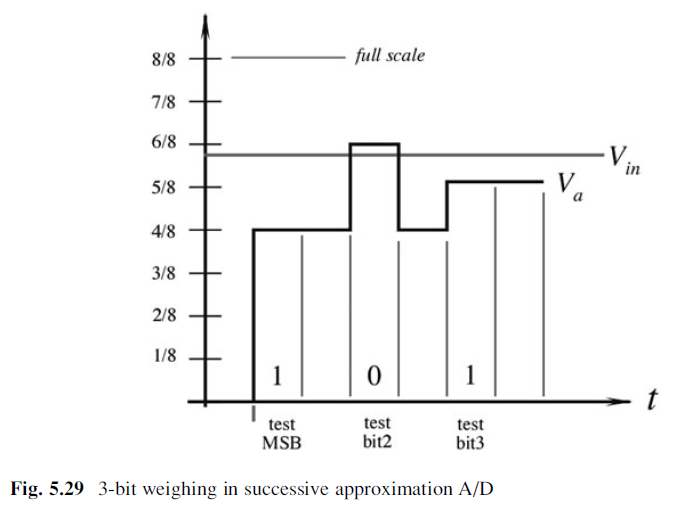
\includegraphics[width =  0.9\textwidth]{L5/img/SAR-graph.PNG}
\end{figure}
\end{minipage}

To make the conversion valid, the input signal $V_{in}$ must not change until all the
bits are tried. To avoid problems, a SAR
is usually supplied with a \textbf{sample and hold} (S\&H) circuit placed just before the comparator (simply made of a switch and a big capacitor). This circuit is a short-time analog memory, which samples the input signal and stores it as a DC voltage during an entire conversion cycle\footnote{A good example can be found on \href{https://www.youtube.com/watch?v=BD3k9bO3hJ0}{https://www.youtube.com/watch?v=BD3k9bO3hJ0}.}. 

\subsubsection{Resolution enhancement}

The input signal $V_m$ has a full-scale value $E$. For a 10-bit converter, the
initial resolution will be $$ R_o = \frac{E}{2^{10} - 1} = \frac{E}{1023} $$
Initially, the multiplexer (MUX) connects the input signal
to the A/D converter, which produces the output digital value $M$, which is
expressed in bits. Then, the microprocessor outputs that value to a D/A converter,
which produces output analog voltage $V_c$, which is an approximation of the input
signal. This voltage is subtracted from the input signal and amplified by the
amplifier to a value $$ V_D = (V_m - V_c) A $$
The voltage $V_D$ is an amplified error between the actual and digitally represented
input signals. The multiplexer connects that voltage to the A/D converter which converts $V_D$ to a
digital value $C$.
As a result, the microprocessor combines two digital values: $M$ and $C$, where
$C$ represents the high resolution bits. The output digital signal is then
\[
    D_{out} = M + C/A
\]
and the extended resolution is
\[
    R = \frac{E}{A\left( 2^{10} - 1 \right)}.
\]

\begin{figure}[H]
    \centering
    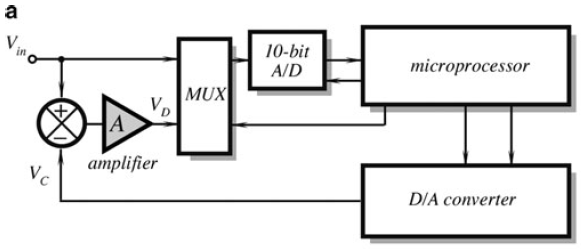
\includegraphics[width =  0.5\textwidth]{L5/img/resolution-extension.PNG}
\end{figure}


\subsubsection{Oversampling and noise power}

The quantization error energy has a fixed
amount of power $V^2_{LSB}/12$ for a given resolution $N$ and is distributed evenly over
the band from 0 to $f_s/2$. After sampling at the Nyquist rate, this spectrum is mirrored into the alias bands and the noise is then spread on all the frequencies. If the sample rate of an analog-to-digital converter is increased from the sample
rate needed to fulfill the Nyquist criterion $f_{s,ny}$ to a new frequency $f_s$, the noise
power density (power per Hz) is reduced with the ratio of the sample rates.
The ratio $$OSR = \frac{f_s}{f_{s,ny}} = \frac{f_s}{2f_b}$$ 
is called the oversampling ratio. The bandwidth BW of the signal is for the
ease of the calculation assumed to range from 0 to $f_b$. Th
noise power density is
$$ \frac{Q^2}{f_s/2} = \frac{V_{LSB}^2/12}{f_s/2} = \frac{V_{LSB}^2}{6f_s}$$
In a band from 0 to $f_b$ the total noise power $Q_b^2$ is found by integrating the noise
density over the band from 0 to $f_b$, resulting in a Nyquist noise power
$$ Q^2_b=  \frac{V_{LSB}^2 f_b}{6f_s} = \frac{V_{LSB}^2}{12} \frac{1}{OSR}$$
The gain in signal-to-noise ratio and in effective number of bits in a fixed
bandwidth is:
\begin{align*}
\Delta SNR & = SNR_b - SNR_{ny} \\
           & = 10 \log\Big(\frac{P_{signal}}{Q_b^2}\Big) - 10 \log\Big(\frac{P_{signal}}{Q^2}\Big) \\
           & = 10 \log\Big(\frac{Q^2}{Q_b^2}\Big) \\
           & = 10 \log\Big(\frac{V_{LSB}^2/12}{\frac{f_{s,ny}}{f_s}V_{LSB}^2/12}\Big) \\
           & = 10 \log\Big(\frac{f_s}{f_{s,ny}}\Big) \\
           & = 10 \log(OSR)
\end{align*}

\begin{figure}[H]
    \centering
    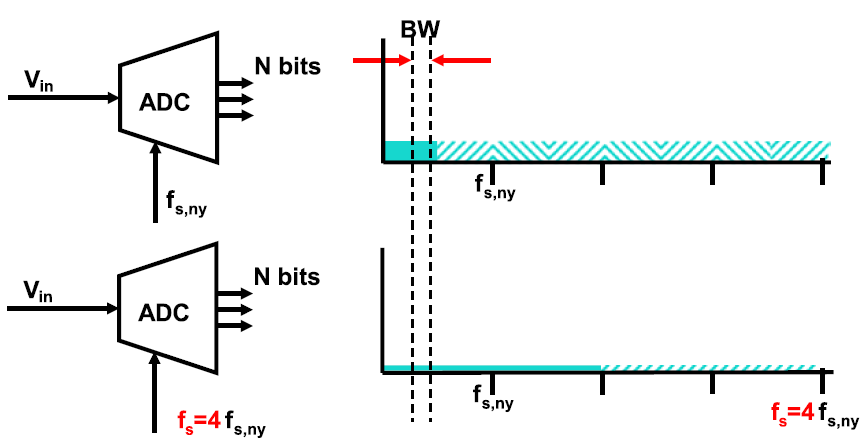
\includegraphics[width = 0.5 \textwidth]{L5/img/oversampling.PNG}
\end{figure}

\paragraph{Advantages}

\begin{itemize}
    \item Oversampling reduces the random white (thermal)
    noise power by OSR (noise voltage $\div \sqrt{OSR}$)
    \item Distribute the quantization noise energy over a
    larger bandwidth
\end{itemize}

\subsubsection{Noise shaping}

\begin{minipage}[c]{0.45 \linewidth}
Noise shaping consists of shifting the quantization energy out of the wanted signal band into
a part of the frequency span where it no longer affects the signal.
\end{minipage}\hfill
\begin{minipage}[c]{0.45 \linewidth}

\begin{figure}[H]
    \centering
    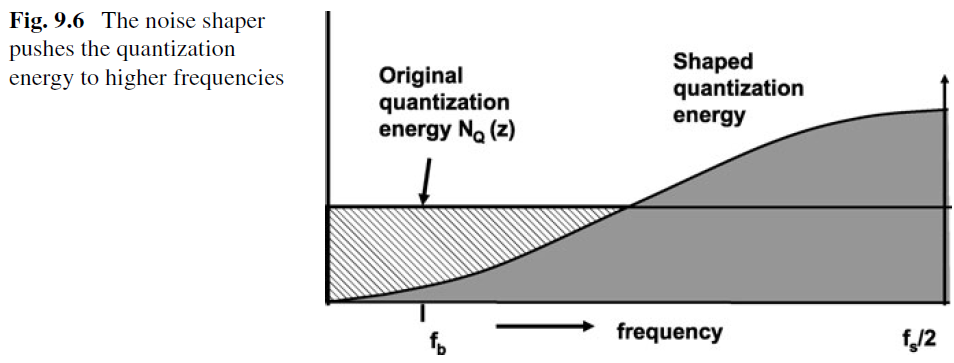
\includegraphics[width =  0.8\textwidth]{L5/img/noise-shaping.PNG}
\end{figure}

\end{minipage}


\paragraph{Advantages}
\begin{itemize}
    \item Cancels the quantization error at DC
    \item Reduces the total quantization noise
\end{itemize}

\paragraph{Remark}

Oversampling and noise shaping allow the use of low resolution but fast components (ideal for modern CMOS technologies).  

\subsubsection{Sigma-Delta ADC}
Integrates (Sigma) the difference (Delta) between the quantized output and the input.

\paragraph{Conclusions}

\begin{itemize}
    \item Digitization features two sub operations: \textbf{sampling }and \textbf{quantization}.
    \item Starting at 7-bit resolution, quantization error behaves similarly as \textbf{thermal noise}.
    \item The main non idealities of ADCs are \textbf{differential} non linearities and \textbf{integral} non linearities.
    \item The basic \textbf{flash} ADC architecture is limited to 8-10 bits due to excessive \textbf{cost} or \textbf{power}.
    \item Successive-approximation ADCs are limited to 16-bit resolution by the \textbf{accuracies} of passive components.
    \item Higher resolution can be reached with specific techniques such as \textbf{resolution enhancement} and $\Sigma \Delta$ ADCs.
\end{itemize}
